\chapter{Les sessions}

Chaque session correspond à un cas d'étude différent. Lorsque le logiciel est utilisé pour analyser une situation inédite, une nouvelle session doit être créée.\\

Une session est caractérisée par un ensemble d'acteurs plus ou moins importants (acteurs principaux et secondaires) et par les deux récits associés à chacun de ces acteurs. De plus, l'utilisateur donner un nom spécifique à chaque acteur afin de faciliter la compréhension des briques (ainsi, un acteur "père" peut être renommé en "M. X" au sein d'une session, ce renommage n'aura un impact qu'à l'intérieur de cette session).\\

\section{Choix de la session}
Lors du lancement du logiciel, l'utilisateur est amené à choisir entre 3 options :\\
\begin{enumerate}
\item Editer l'ensemble des schémas : Cela correspond à une session générée automatiquement. Elle correspond à la sélection de tous les acteurs possibles. Cette session permet d'avoir une vue globale des situations schématisées dans le logiciel.
\item Créer une nouvelle session : Lance le processus de création d'une session.
\item Ouvrir une ancienne session : La liste des sessions précédentes se situe juste au dessous de cette option. Un double clique sur la ligne d'une ancienne session permet de l'ouvrir automatiquement.
\end{enumerate}

\begin{figure}[h!]
\centering
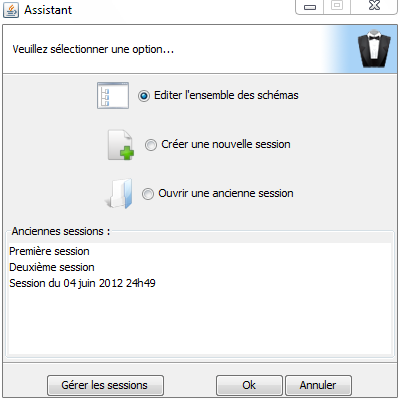
\includegraphics[scale=0.55]{images/ouverture_session.png}

\caption{L'assistant de choix de la session}
\end{figure}

\section{Création d'une nouvelle session}
La première chose à faire lors de la création d'une session est de nommer cette dernière. Cela se fait à l'aide du cadre "Nom de la session".\\

Ensuite, il faut ajouter les acteurs concernés. Pour cela, il faut sélectionner un acteur dans l'arborescence située sur la gauche de la fenêtre puis cliquer sur un des boutons "Ajouter un acteur principal" ou "Ajouter un acteur secondaire". Il est toujours possible par la suite de changer le type d'un acteur sélectionné.\\

Lorsqu'un acteur a ainsi été ajouté, il apparaît dans la liste correspondante ("Acteurs principaux" ou "Acteurs secondaires"). Chaque ligne correspond à un acteur. Il est possible :\\
\begin{itemize}
\item de supprimer l'acteur de la liste (petite croix juste avant le nom)
\item de renommer cet acteur pour la session
\item d'accéder à sa fiche (voir paragraphe \ref{fiche_acteur})
\item de changer le type de l'acteur (principal ou secondaire)\\
\end{itemize}



\begin{figure}[h!t]
\centering
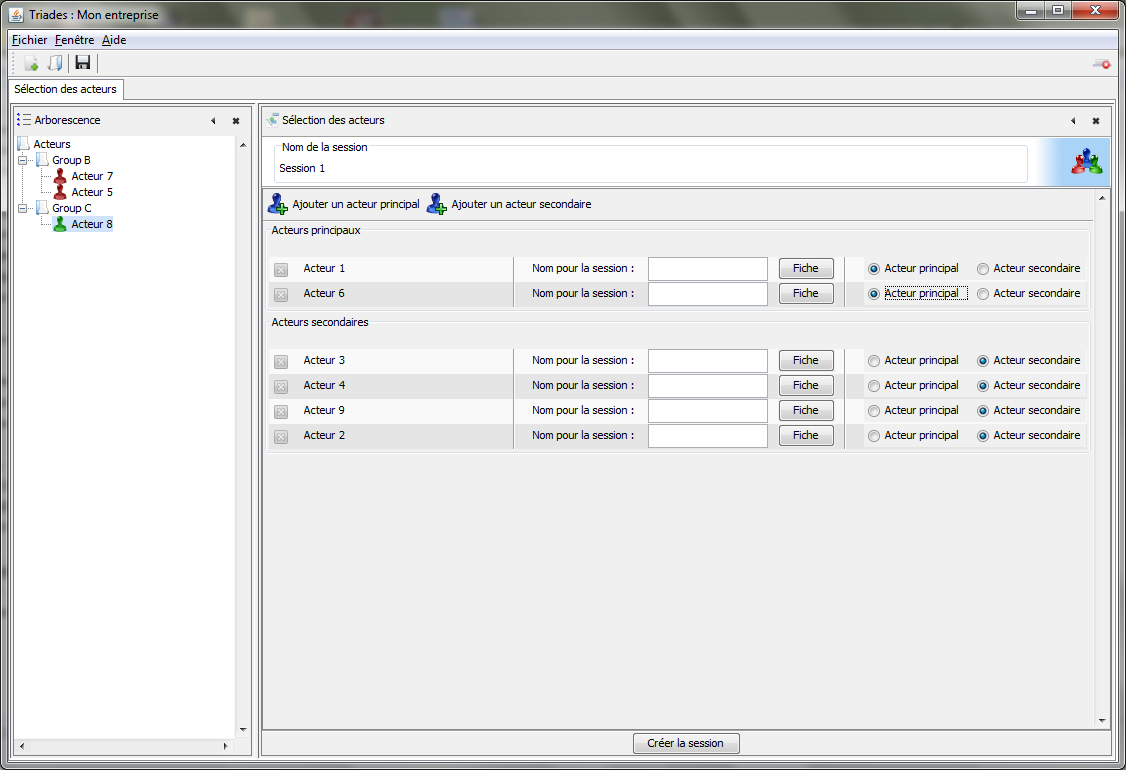
\includegraphics[scale=0.35]{images/selection_acteurs.png}

\caption{Création d'une nouvelle session, sélection des acteurs}

\end{figure}

Une fois la liste finalisée, il suffit de cliquer sur le bouton correspondant en bas de la fenêtre pour créer la session. Attention, il n'est plus possible de modifier la liste des acteurs une fois la session créée.\\

\section{Fiches des acteurs}
\label{fiche_acteur}
Chaque acteur est associé à une fiche. Elle permet de saisir les deux récits et de changer le nom associé à l'acteur. Chaque fiche est liée à une seule session (les récits saisis dans une session ne seront pas accessible depuis une autre). De plus un résumé de la situation de l'acteur est disponible à la suite des zones de texte.\\

Il est possible de revenir au nom par défaut d'un acteur en supprimant complètement le texte dans le champ "Nom associé à l'acteur "..." pour la session".\\

Les zones de textes "Premier récit", "Deuxième récit" et "Notes" permettent de saisir des informations concernant cet acteur.\\

La partie suivante présente un résumé de la situation de l'acteur, en triant les briques en fonctions des relations qui concernent cet acteur. En premier sont placés les briques présentant au moins une relation en écart, puis au moins une relation incomplète, et enfin celles n'ayant que des relations en accord. Il est possible d'accéder directement à une brique en cliquant sur son nom.\\

\begin{figure}[h!t]
\centering

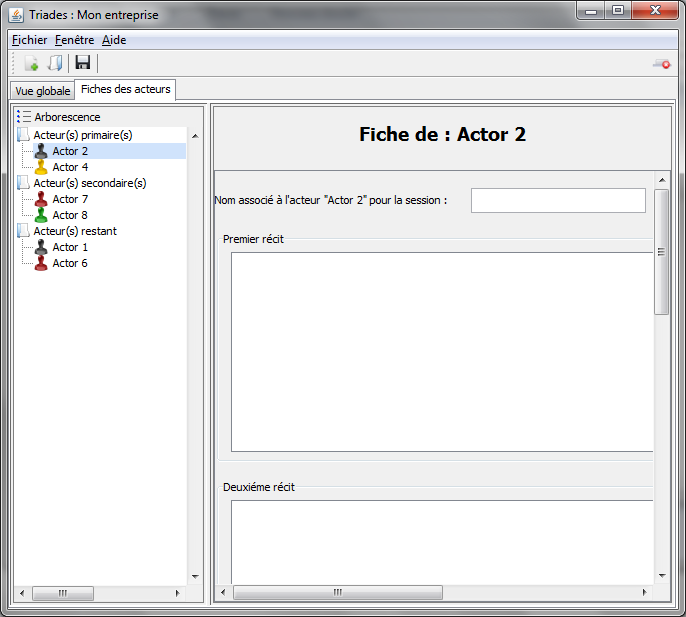
\includegraphics[width=12cm]{images/fiche_acteur.png}

\caption{La fiche d'un acteur}

\end{figure}

Il possible d'accéder à la fiche d'un acteur en faisant un clic droit sur ce dernier. Cela peut être fait dans un arbre ou dans une brique (voir figure~\ref{menu_fiche_acteur}). De plus l'arbre présent sur la gauche de la fiche d'un acteur permet d'accéder rapidement à l'ensemble des acteurs présent dans la sessions. La catégorie acteur restant correspond aux acteurs présent dans une brique mais n'ayant pas été sélectionné par l'utilisateur. Ces acteurs ne sont disponibles qu'une fois la session créée.\\

L'onglet "Liste des acteurs" permet à tout moment de retourner à l'affichage des fiches des acteurs.


\begin{figure}[h!t]
\centering
\Ovalbox{
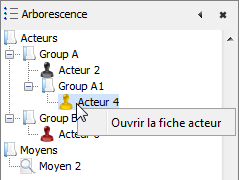
\includegraphics[width=6cm]{images/menu_fiche_acteur.png}
}

\caption{Le menu contextuel permettant d'ouvrir la fiche d'un acteur}

\label{menu_fiche_acteur}
\end{figure}

\section{Interface de gestion des sessions}
Cette interface est accessible depuis l'écran d'acceuil de \tria. Elle permet de gérer l'ensemble des sessions courantes. Les actions possibles sont :\\
\begin{itemize}
\item \textbf{Ouvrir} : Permet d'ouvrir la session sélectionnée. Si plusieurs sessions sont sélectionnées, un message d'erreur apparaît.\\
\item \textbf{Archiver} : Permet d'archiver des sessions dans un fichier. Ces sessions sont ensuite supprimées de la liste des sessions courantes.\\
\item \textbf{Sauvegarder sous} : Permet d'enregistrer une copie des sessions sélectionnées dans un fichier. Ces sessions sont conservées dans la liste des sessions courantes.\\
\item \textbf{Importer} : Permet d'ajouter à la liste des sessions courantes les sessions d'un fichier. Si une session portant le même nom qu'une session importée est déjà présente dans la liste, il sera demandé à l'utilisateur s'il veut remplacer la session présente dans la liste. Attention, en cas de remplacement, cette session sera perdue.\\
\item \textbf{Renommer} : Permet de renommer les sessions sélectionnées. Il est possible de renommer plusieurs sessions à la suite en faisant une sélection multiple.\\
\item \textbf{Supprimer} : Permet de supprimer des sessions. Attention, cette opération est irréversible.\\
\end{itemize}

Il est possible de sélectionner plusieurs sessions en même temps afin d'exporter dans un même fichier un ensemble de sessions. Pour cela la touche \textit{Ctrl} permet d'ajouter un élément à la sélection, et \textit{Maj} permet de sélectionner un groupe de sessions.\\

\begin{figure}[h!]
\centering
\Ovalbox{
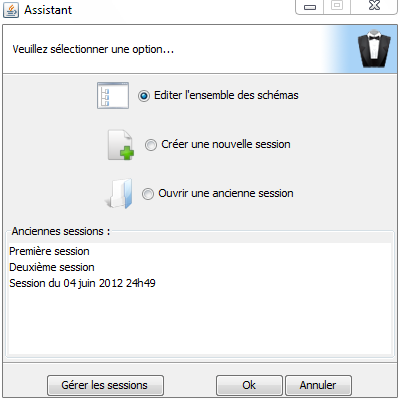
\includegraphics[width=0.6\textwidth]{images/ouverture_session.png}
}
\caption{L'interface de gestion des sessions\\est accesible depuis l'assistant d'ouverture}

\end{figure}
~
\begin{figure}[h!]
\centering
\Ovalbox{
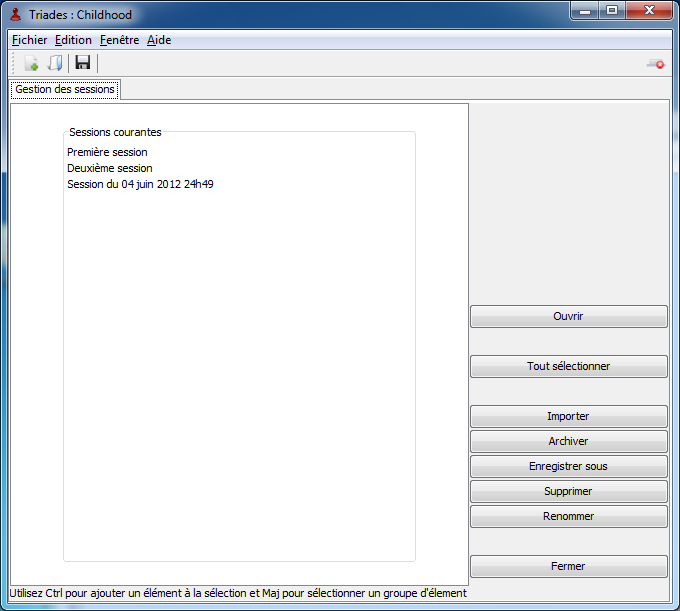
\includegraphics[width=0.8\textwidth]{images/gestion_session.png}
}
\caption{L'interface de gestion des session}
\end{figure}